% 2012_tianjin_science_q17_fig1: schematic pyramid P-ABCD, PA vertical
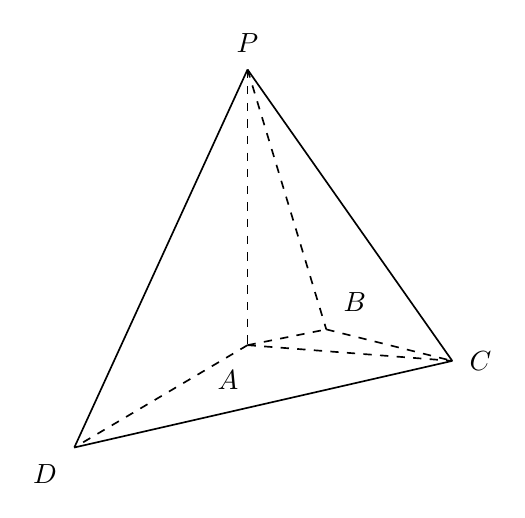
\begin{tikzpicture}[x=1cm,y=1cm,font=\normalsize,line width=.6pt]
\coordinate (P) at (0,5.0);
\coordinate (A) at (0,1.5);
\coordinate (B) at (1.0,1.7);
\coordinate (C) at (2.6,1.3);
\coordinate (D) at (-2.2,0.2);
% solid visible edges
\draw[solid] (P) -- (D);
\draw[solid] (P) -- (C);
\draw[dashed] (B) -- (C);
\draw[solid] (C) -- (D);
% hidden edges
\draw[dashed] (P) -- (A);
\draw[dashed] (P) -- (B);
\draw[dashed] (A) -- (B);
\draw[dashed] (A) -- (C);
\draw[dashed] (A) -- (D);
% labels with clearance
\node[inner sep=2pt,above=4pt] at (P) {$P$};
\node[inner sep=2pt,below left=4pt,xshift=3pt,yshift=-3pt] at (A) {$A$};
\node[inner sep=2pt,above right=4pt] at (B) {$B$};
\node[inner sep=2pt,right=4pt] at (C) {$C$};
\node[inner sep=2pt,below left=4pt] at (D) {$D$};
\end{tikzpicture}
